\begin{voorstel}{De rol van de RES}
\meeschrijver{Walter Wittkamp}

\headerimg[][\copyright{} Mike Moore \CC{} 0]{img/energie/rol-van-de-res-header}
% https://commons.wikimedia.org/wiki/File:FEMA_-_32463_-_SBA_at_Findlay_Town_Meeting_in_Ohio.jpg
% TODO: get a picture of a real citizens assembly!

\begin{samenvatting}
In de Regionale Energiestrategieën moet burgerparticipatie voorop staan om de burger eigenaar van de transitie te maken. Burgerberaden zullen een belangrijke rol spelen om tot adequaat, haalbaar en rechtvaardig klimaatbeleid te komen.
\end{samenvatting}

\begin{multicols*}{2}

\begin{uitdaging}
In het klimaatakkoord zijn dertig energieregio’s opgericht waar provincies, gemeenten en waterschappen een plan maken over de vergroening van de energievoorziening van hun regio. In deze Regionale Energiestrategieën (RES) ligt de nadruk op duurzame elektriciteit uit zon en wind, verwarming van gebouwen, en alle infrastructuur die daarvoor nodig is. De conceptvoorstellen zijn eind 2020 door elke regio ingediend, nu moet de gemeente aan de slag.
Participatie van inwoners heeft in dit proces echter nog nauwelijks plaatsgevonden. En de tot nu toe gepresenteerde plannen zijn niet ambitieus en dwingend genoeg om de klimaatcrisis aan te pakken.
Hoe zorgen we ervoor dat burgers inspraak krijgen op de regionale strategievorming? En hoe brengen we de urgentie van de klimaatcrisis in het beleid?
\end{uitdaging}

\begin{overwegingen}

\paragraph{De urgentie mist}
De gepresenteerde RES'en geven vooral invulling aan de in het klimaatakkoord gestelde doelen over de hoeveelheid duurzaam op te wekken elektriciteit.
Zowel in het klimaatakkoord als in de RES'en lijkt het hoofddoel van ambitieus klimaatbeleid echter buiten beeld te blijven: reageren op klimaatverandering en het bouwen van een toekomstbestendige wereld. Bij het opstellen van het klimaatakkoord was dan ook geen enkele wetenschappelijke expert betrokken \parencite{kropman_hoe_2019}.

Het gestelde doel voor elektriciteit was om in 2030 landelijk 35 terawattuur (TWh) stroom op te wekken met zonnedaken, zonneweides en windparken op het Nederlandse vasteland. Dat is circa 30 procent van het huidige landelijke stroomverbruik.
Door de verwachting dat het elektriciteitsverbruik de komende jaren zal stijgen, is de ambitie binnen de RES echter te laag.
Daarnaast lukken ook niet alle plannen altijd, door bijvoorbeeld technische beperkingen en tegenslag, juridische procedures, gebrek aan interesse bij ondernemers, problemen met vergunningen of door een tekort aan vakspecialisten.

Er zijn nu geen maatregelen of sancties als men niet aan de opgave voldoet.
Nederland doet het al het slechtst van alle landen in Europa wat betreft duurzame energie en is één van de grootste vervuilers per hoofd van de bevolking. Doordat er de afgelopen jaren nauwelijks tot concrete actie is overgegaan binnen de RES, maar vooral is overlegd, raakt Nederland nog verder achterop.

\begin{figure}[H]
	\begin{center}
		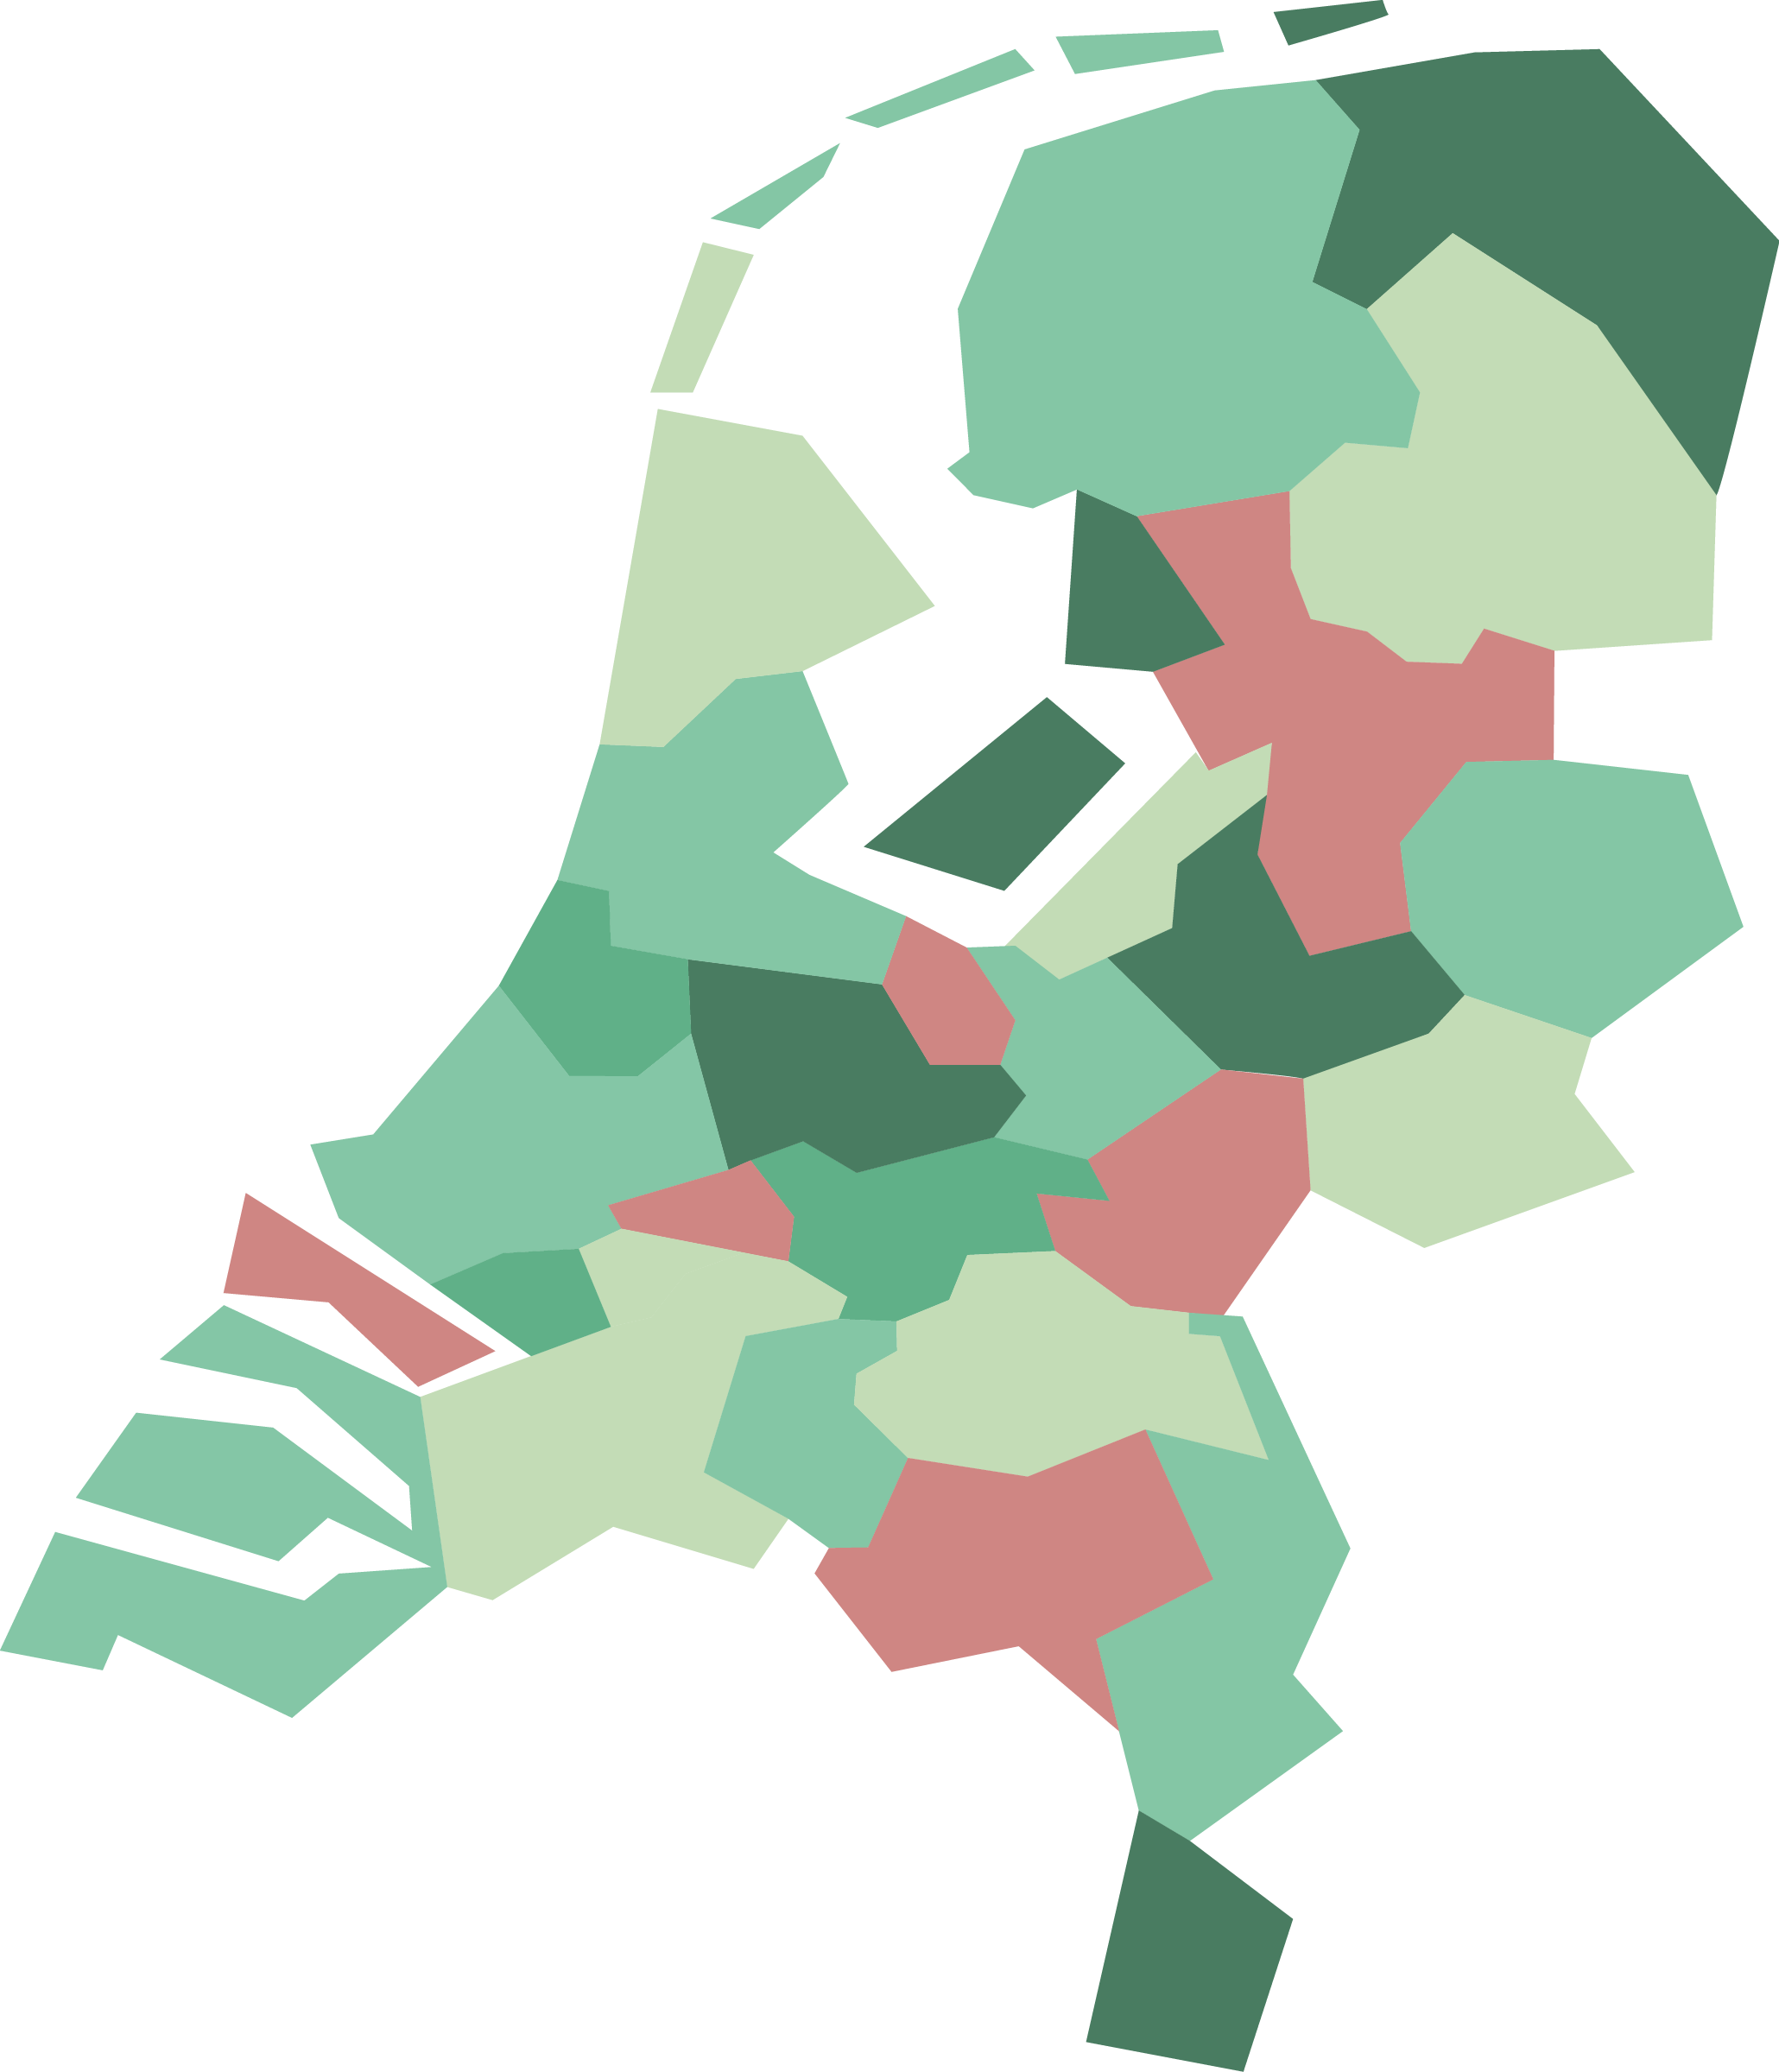
\includegraphics[width=.8\columnwidth]{img/energie/rol-van-de-res-kaart}
	\end{center}
	\textbf{\textit{Kaart met de 30 regio's \parencite{nationaal_programma_res_handreiking_2019}.}}
\end{figure}

\paragraph{Gebrek aan overkoepelende visie}
In de RES’en wordt voorbijgegaan aan het complexe vraagstuk dat klimaatverandering voor een regio is. Er zijn afhankelijkheden tussen de regio’s, bijvoorbeeld in het gebruik van restwarmte van de industrie over regiogrenzen heen. Er zijn ook gerelateerde vraagstukken: de afname van biodiversiteit, toenemende woningnood, verduurzaming van de landbouw en voedselindustrie, Europese verplichtingen, en het stikstof-dossier. De gemeenten lijken de visie te missen om de RES als overkoepelend instrument te gebruiken om de klimaatcrisis tegen te gaan.

\paragraph{Draagvlak ontbreekt}
Het draagvlak voor de RES-beslissingen van provincies en gemeenten is minimaal, zeker bij de inwoners. Er was in het RES-proces weinig invloed van de volksvertegenwoordigers in de gemeenteraden \parencite{prins_eis_2020}. De inwoners, die dit moeten betalen en de gevolgen zullen merken, zijn tot nu toe nauwelijks betrokken. De RES’en zijn vooral ideeën van bestuurders, ambtenaren en ondernemers.

\paragraph{Hoe het anders kan}
Er zijn in Nederland gelukkig inspirerende voorbeelden hoe de besluitvorming anders kan.
Zo is in de gemeente Wijk bij Duurstede het beleid voor zonnevelden via een open proces opgesteld. Er ontstond een mooi voorbeeld van samenspel tussen inwoners en volksvertegenwoordigers. Een burgerpanel, samengesteld door loting met een evenredige verdeling over de drie kernen in het betreffende gebied, heeft de gemeenteraad geadviseerd over het te voeren energiebeleid. Dit advies is vervolgens door de raad overgenomen en vormt daarmee het kader waarbinnen voorstellen voor concrete projecten ingediend kunnen worden bij de gemeente \parencite{burgerpanel_zonnevelden_wijk_bij_duurstede_advies_2019}.
In Kampen vond een energietop plaats voor inwoners, bedrijven en raadsleden. En in de regio Drechsteden waren er waren regionale bijeenkomsten waar volksvertegenwoordigers, inwoners, bedrijven en stakeholders met elkaar in gesprek konden over energiescenario’s.

\todo{
\paragraph{Over de grens}
Franse burgerconventie

De Franse burgerconventie over het klimaat laat zien dat het mogelijk is om gedegen klimaatbeleid te ontwikkelen (NRC 2020-2). Het beraad maakt gebruik van democratie in de volle breedte en zorgt dat alle kennis, creativiteit en verantwoordelijkheidsgevoel in de samenleving wordt benut. Laten we het Franse voorbeeld (en dat van Wijk bij Duurstede) volgen. We doorbreken zo de impasse rond klimaatbeleid en maken onze democratie geschikt voor de eenentwintigste eeuw.

% \url{https://www.nrc.nl/nieuws/2020/07/03/laat-burgers-politici-helpen-organiseer-een-burgerberaad-a4004913#/handelsblad/2020/07/04/#204} (NRC 2020-2)
}

\paragraph{De waarde van burgerberaden}
Burgerberaden zijn een uitermate geschikt instrument om participatie en inspraak van burgers over het energiebeleid vorm te geven.
De beraden stellen over het algemeen adequate, haalbare en rechtvaardige maatregelen voor. De deelnemers vertegenwoordigen immers geen politieke partij en hoeven dus geen rekening te houden met verkiezingen, gunstige media-aandacht of een achterban. Partijpolitiek en lobbygroepen hebben weinig tot geen invloed op de besluitvorming van het burgerberaad, onder andere doordat de uitvoering in handen is van een onafhankelijke organisatie. En anders dan bij een referendum of enquête staat deliberatie centraal. Dat zorgt ervoor dat mensen voorbij ideologische, culturele en religieuze verschillen leren kijken en afgaan op feiten. De deelnemers krijgen tijd, informatie van experts en professionele gespreksbegeleiding, wat ze helpt in gesprek te gaan over complexe onderwerpen en tot constructieve, weldoordachte aanbevelingen te komen.
\todo{Hiermee geven we een invulling aan Remkes \parencite{staatscommissie_parlementair_stelsel_lage_2018}}

\todo{balans nationaal-regionaal. Hoe houden we nationaal overzicht en regionaal handelingsperspectief?}

\end{overwegingen}

\begin{aanbevelingen}
\speerpunt{We stellen een Nationaal Klimaatberaad in} om klimaatmaatregelen vast te stellen die ons beschermen tegen een onnodige verdere stijging van de temperatuur en de potentieel catastrofale gevolgen daarvan.

\speerpunt{We stellen regionale burgerberaden in} om voorstellen voor de regionale energietransitie op te stellen.

\end{aanbevelingen}

\end{multicols*}

\end{voorstel}
